%\documentclass[handout]{beamer}
\documentclass{beamer}
\usepackage{algorithm2e}
\usepackage{natbib}
\usepackage{layouts}
%\usepackage{enumitem}
%\usepackage[dvipsnames]{xcolor}
\definecolor{vuborange}{rgb}{1.0,0.40,0.0}
\usetheme{Boadilla}
\usepackage{color,soul}
\usepackage{xcolor}
\usepackage{adjustbox}
\usepackage{amsmath,amssymb}
\usepackage{tikzsymbols}
\usepackage{booktabs}
\usepackage{calc}
\usepackage{tikz}
\usepackage{tikz-qtree}

%\newcommand\citet[1]{\citeauthor{#1}~\citeyear{#1}}
\usepackage[bordercolor=white,backgroundcolor=gray!30,linecolor=black,colorinlistoftodos]{todonotes}
\newcommand{\rework}[1]{%
	\todo[color=yellow,inline]{Rework: {#1}}%
}

\usetikzlibrary{shapes.geometric, arrows}

\title{Efficiently Explaining CSPs with Unsatisfiable Subset Optimization}
\institute[shortinst]
{\inst{1} Vrije Universiteit Brussel, Belgium \\ % Your institution for the title page
	\inst{2} KULeuven, Belgium \\ % Your institution for the title page
	\href{mailto:emilio.gamba@vub.be}{\underline{emilio.gamba@vub.be}}, \href{mailto:bart.bogaerts@vub.be}{bart.bogaerts@vub.be}, \href{mailto:tias.guns@kuleuven.be}{tias.guns@kuleuven.be} % Your email address
}
\date{EURO 2022}
\author{\underline{Emilio Gamba}\inst{1} \and  Bart Bogaerts\inst{1} \and   Tias Guns\inst{1,2}}

\newcommand\hlyellow[1]{\hl{ {\sethlcolor{yellow}#1}}}
\newcommand\hlgreen[1]{\sethlcolor{green}\hl{#1}}

\tikzstyle{startstop} = [rectangle, rounded corners, minimum width=2cm, minimum height=0.5cm,text centered, draw=black]
\tikzstyle{io} = [trapezium, trapezium left angle=70, trapezium right angle=110, minimum width=3cm, minimum height=1cm, text centered, draw=black, fill=blue!30]
\tikzstyle{process} = [rectangle, minimum width=3cm, minimum height=1cm, text centered, draw=black, fill=orange!30]
\tikzstyle{decision} = [diamond, minimum width=3cm, minimum height=1cm, text centered, draw=black, fill=green!30]
\tikzstyle{arrow} = [thick,->,>=stealth]


\newcommand\m[1]{\ensuremath{\mathcal{#1}}\xspace}
\newcommand\allconstraints{\m{T_P}}
\newcommand\theory{\ensuremath{\m{F} }\xspace}
\newcommand\formula{\ensuremath{\m{F} }\xspace}
\newcommand\formulac{\ensuremath{\m{C} }\xspace}
\renewcommand\emph[1]{{\color{vuborange}#1}}
\newcommand\Iend{\m{I_{\mathit{end}}}}
\newcommand\Ipartial{\m{I}}
\newcommand\factexpl{fact\xspace}
\newcommand\LitsToExplain{FactsToExplain}

\newcommand\nat{\m{\mathbb{N}}}
\newcommand\subsetT{\m{\mathcal{S}}}
\newcommand\ltrue{\m{\textbf{t}}}
\newcommand\lfalse{\m{\textbf{f}}}
\newcommand\call[1]{\m{\textsc{#1}}}
\newcommand\onestep{\call{OneStep}}

\newcommand\muses[1]{\textsc{mus}s(\m{#1})}
\newcommand\mcses[1]{\textsc{mcs}s(\m{#1})}
%\begin{frame}{How to find OCUSs?}
%
%	
%\end{frame}

\newcommand\setstohit{\m{\mathcal{H}}}
\newcommand\grow{\call{Grow}}
\newcommand\sat{\call{SAT}}
\newcommand\corrss{\call{Correction-Subsets}}
\newcommand\comus{\call{ocus}}
\newcommand\cohs{\call{cost-optimal-hittingset}}
% \renewcommand{\labelitemi}{$\triangleright$}
\renewcommand{\thealgocf}{}


\makeatletter
\renewcommand{\@algocf@capt@plain}{above}% formerly {bottom}
\setbeamertemplate{footline}
{
	\leavevmode%
	\hbox{%
		\begin{beamercolorbox}[wd=.2\paperwidth,ht=2.25ex,dp=1ex,center]{author in head/foot}%
			\usebeamerfont{author in head/foot}Emilio Gamba (VUB)
		\end{beamercolorbox}%
		\begin{beamercolorbox}[wd=.6\paperwidth,ht=2.25ex,dp=1ex,center]{title in head/foot}%
			\usebeamerfont{title in head/foot}Efficiently Explaining CSPs with Unsatisfiable Subset Optimization
		\end{beamercolorbox}%
		\begin{beamercolorbox}[wd=.2\paperwidth,ht=2.25ex,dp=1ex,right]{date in head/foot}%
			\usebeamerfont{date in head/foot}August 2021\hspace*{1em}
			\insertframenumber{} / \inserttotalframenumber\hspace*{2ex} 
	\end{beamercolorbox}}%
	\vskip0pt%
}
\makeatother

\begin{document}
	
	\begin{frame}
		\maketitle
	\end{frame}
	
	
	\AtBeginSection[]
	{
		\begin{frame}
			\frametitle{Outline}
			\tableofcontents[currentsection]
		\end{frame}
	}
	
	\AtBeginSubsection[]
	{
		\begin{frame}
			\frametitle{Outline}
			\tableofcontents[currentsection,currentsubsection]
		\end{frame}
	}
	
	\begin{frame}
		
		\setlength{\textfloatsep}{0pt}
		\frametitle{Examples of Constraint Satisfaction Problems}
		\begin{minipage}[t]{0.45\textwidth}
			\begin{figure}[h]
				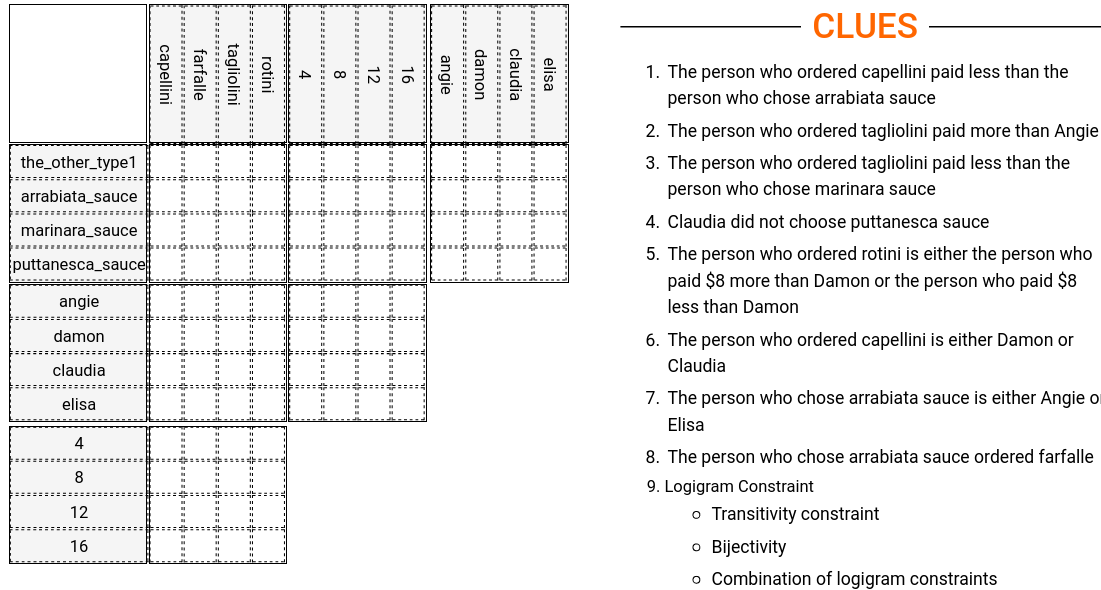
\includegraphics[width=\textwidth]{figures/logic_puzzle.png}
				\vspace{-8mm}
				\caption{\small Logic Grid Puzzle}
			\end{figure}
			\vspace{-6mm}\pause
			\begin{figure}[h]
				\centering
				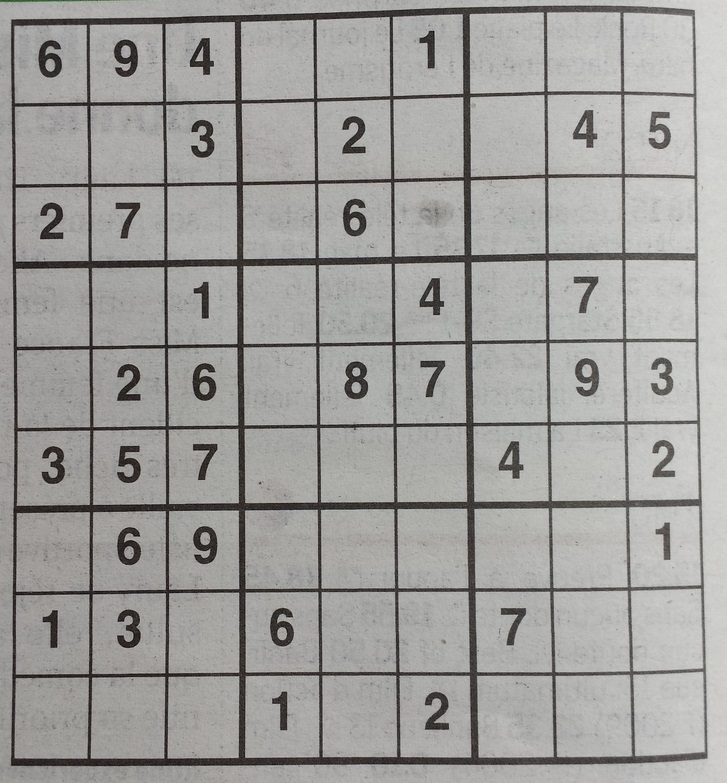
\includegraphics[width=.5\textwidth]{figures/sudoku.jpg}
				\vspace{-3mm}
				\caption{\small Sudoku}
			\end{figure}
		\end{minipage}\pause
		\hfill
		\begin{minipage}[t]{0.45\textwidth}
			\begin{figure}[h]
				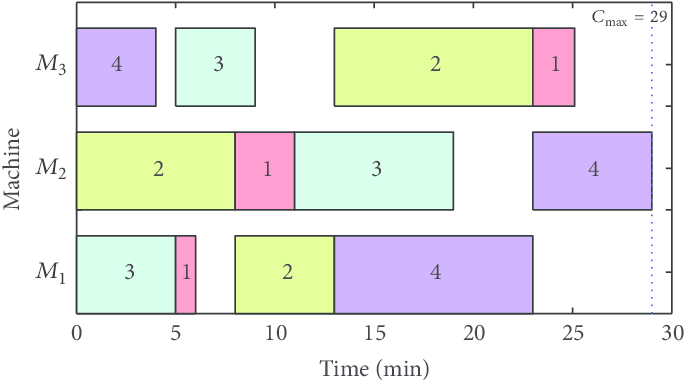
\includegraphics[width=\textwidth]{figures/scheduling.png}
				\vspace{-9mm}
				\caption{\small Scheduling Problem}
			\end{figure}
			\vspace{-6mm}\pause
			\begin{figure}[h]
				\includegraphics[width=\textwidth]{figures/omus-presentation-car.png}
				\vspace{-9mm}
				\caption{\small Configuration problems}
			\end{figure}
		\end{minipage}
		\footnote{\tiny \url{https://www.researchgate.net/figure/The-schedule-of-4-3-job-shop-scheduling-problem_fig2_301279276}}
	\end{frame}
	

\begin{frame}
	\frametitle{Constraint Satisfaction Problems}
	\framesubtitle{Solving}
	
	\begin{center}
		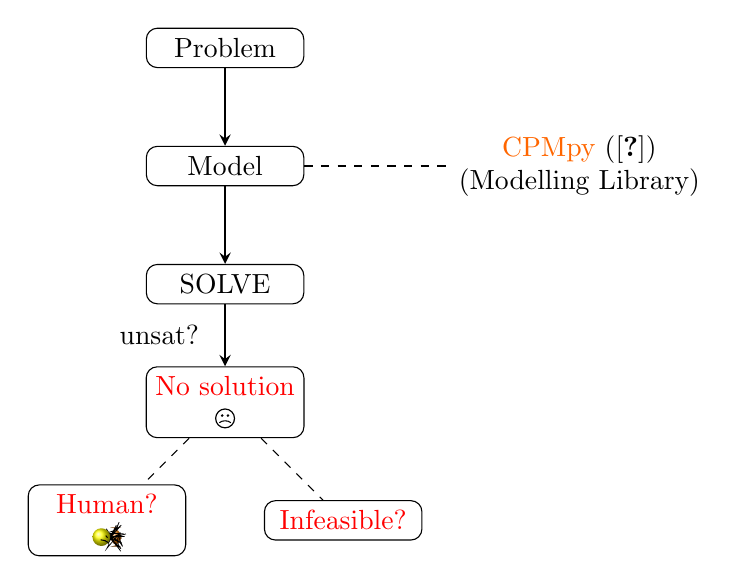
\begin{tikzpicture}[node distance=1.5cm]
			\node (problem) [startstop] {Problem};
			
			\node (model) [startstop, below of=problem] {Model}; 
			\draw [arrow] (problem) -- (model);			
%			\node (Essence) [right of=model, xshift=1cm] {CPMpy \cite{CPMpy}}; 
			\node (cpmpy) [align=center, right of=model, xshift=3cm] {\emph{CPMpy} (\cite{guns2019increasing}) \\ (Modelling Library)}; 
%			\node (Essence) [right of=model, xshift=1cm] {CPMpy \cite{CPMpy}}; 
			\draw [dashed] (model) -- (cpmpy);									
			\pause
			
			\node (solve) [startstop, below of=model] {SOLVE};
			\draw [arrow] (model) -- (solve); \pause
			
			\node  (modelerror) [startstop, below of=solve, align=center] {\color{red} No solution\\ \Sadey}; %todo: add smiley face sad
			\draw [arrow] (solve) --node[anchor=east,xshift=-0.2cm] {unsat?} (modelerror); 			
			\pause
			\node  (human) [startstop, below of=modelerror, xshift=-1.5cm, align=center] {\color{red} Human?\\\drWalley}; %todo: doodle human
			\draw [dashed] (modelerror) --  (human); 
			\pause
			\node  (Infeasible) [startstop, below of=modelerror, xshift=1.5cm, align=center] {\color{red} Infeasible?}; 
			\draw [dashed] (modelerror) --  (Infeasible); 

		\end{tikzpicture}
	\end{center}
\end{frame}

\begin{frame}
	\frametitle{Constraint Satisfaction Problems}
	\framesubtitle{Solving}
			\begin{minipage}{0.4\textwidth}
		\begin{center}
			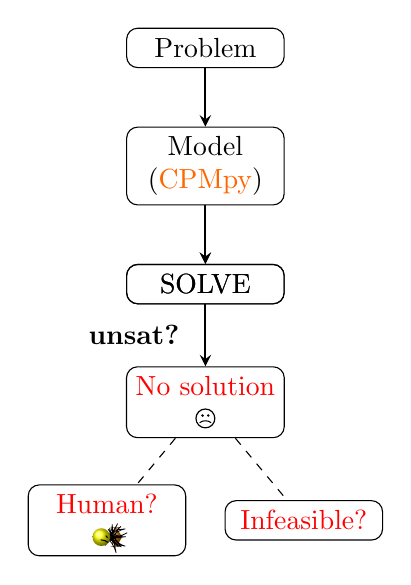
\begin{tikzpicture}[node distance=1.5cm]
				\node (problem) [startstop] {Problem}; 
				
				\node (model) [startstop, below of=problem,align=center] {Model \\ (\emph{CPMpy})}; 
				\draw [arrow] (problem) -- (model);			
				
%				\node (cpmpy) [right of=model, xshift=0.75cm] {CPMpy}; 
%				\draw [dashed] (model) -- (cpmpy);									
				
				\node (solve) [startstop, below of=model] {SOLVE};
				\draw [arrow] (model) -- (solve); 
			
			\node (solve) [startstop, below of=model] {SOLVE};
			\draw [arrow] (model) -- (solve); 

			\node  (modelerror) [startstop, below of=solve, align=center] {\color{red} No solution\\ \Sadey}; %todo: add smiley face sad
			\draw [arrow] (solve) --node[anchor=east,xshift=-0.2cm] {\textbf{unsat?}} (modelerror); 			
			\node  (human) [startstop, below of=modelerror, xshift=-1.25cm, align=center] {\color{red} Human?\\\drWalley}; %todo: doodle human
			\draw [dashed] (modelerror) --  (human); 
			\node  (Infeasible) [startstop, below of=modelerror, xshift=1.25cm, align=center] {\color{red} Infeasible?}; 
			\draw [dashed] (modelerror) --  (Infeasible); 

				\end{tikzpicture}
		\end{center}
	\end{minipage}
	\begin{minipage}{0.59\textwidth}
	
	\textbf{How do you explain UNSAT ? }	
	\begin{itemize}
		\item Enumerate \emph{Unsatisfiable Cores} / \emph{Minimum Unsatisfiable Subsets} (MUS) \pause
		\item Extract \emph{Minimum Correction Subsets} (MCS)
		\begin{itemize}
			\item \emph{Correct} your model by modifying a subset of the model constraints
		\end{itemize}
	\end{itemize}
	\end{minipage}
\end{frame}
	
	
	\begin{frame}
		\frametitle{Motivation}
		\framesubtitle{Explaining SAT problems}
		
		\begin{minipage}{0.4\textwidth}
			\begin{center}
				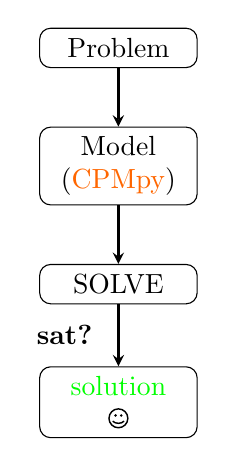
\begin{tikzpicture}[node distance=1.5cm]
					\node (problem) [startstop] {Problem}; 
					
				\node (model) [startstop, below of=problem,align=center] {Model \\ (\emph{CPMpy})}; 
				\draw [arrow] (problem) -- (model);								
					
					\node (solve) [startstop, below of=model] {SOLVE};
					\draw [arrow] (model) -- (solve); 
					
					%					\node  (modelerror) [startstop, below of=solve] {\color{red} modeling error?};
					%					\draw [arrow] (solve) --node[anchor=east,xshift=-0.2cm] {unsat?} (modelerror); 
					\node  (solution) [startstop, below of=solve,align=center]  {\color{green} solution\\ \Smiley};
					%						\node  (solution) [startstop, below of=sat] {\color{green} solution};
					%	
					\draw [arrow] (solve) --node[anchor=east,xshift=-0.2cm] {\textbf{sat?}} (solution);
					
					%						\draw [arrow] (sat) -- (solution);			
					
				\end{tikzpicture}
			\end{center}
		\end{minipage}
		\begin{minipage}{0.59\textwidth}
			
			\textbf{How do I explain SAT ? }	
			\begin{itemize}
				\item What is an \textbf{\emph{explanation}}? \pause
				\item What is a \emph{\textbf{good}} explanation ? 
				\item What is a \textbf{\emph{sequence of explanations}} ? \pause
			\end{itemize}
		\end{minipage}
		
	\end{frame}
	
	
%	\begin{frame}
%		\frametitle{Outline}
%		\tableofcontents
%	\end{frame}
%	
	\section{Stepwise explanations for CSPs}
	\begin{frame}{Stepwise explanations for CSPs}
	\framesubtitle{EXPLANATION STEP}

			\only<1>{
				\begin{figure}[H]
					\centering
				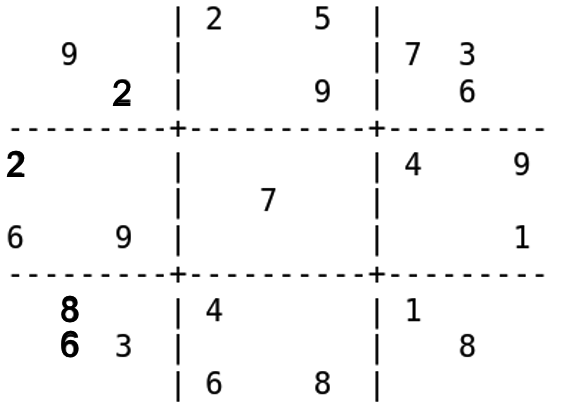
\includegraphics[width=0.8\textwidth]{figures/sudoku-step1}
				\end{figure}
			}
					\only<2>{
				\begin{figure}[H]
	\centering
	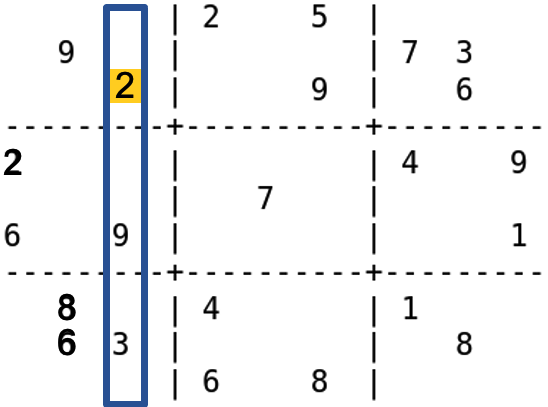
\includegraphics[width=0.8\textwidth]{figures/sudoku-step2}
\end{figure}
		}
				\only<3>{
				\begin{figure}[H]
	\centering
	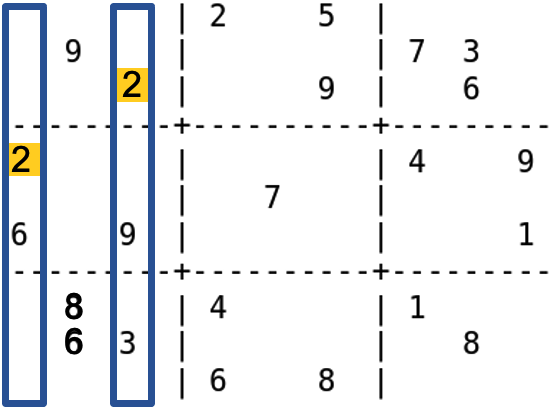
\includegraphics[width=0.8\textwidth]{figures/sudoku-step3}
\end{figure}
	}
			\only<4>{
				\begin{figure}[H]
	\centering
	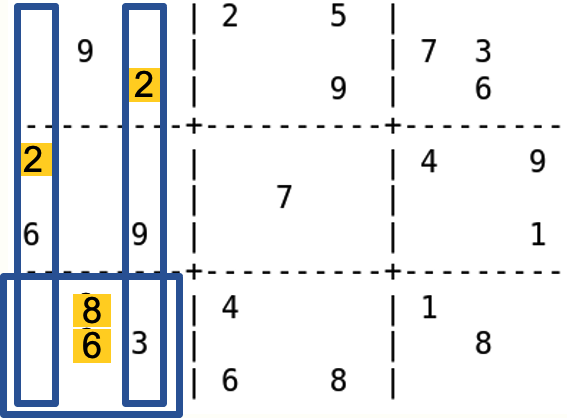
\includegraphics[width=0.8\textwidth]{figures/sudoku-step4}
\end{figure}
}
			\only<5>{
				\begin{figure}[H]
	\centering
	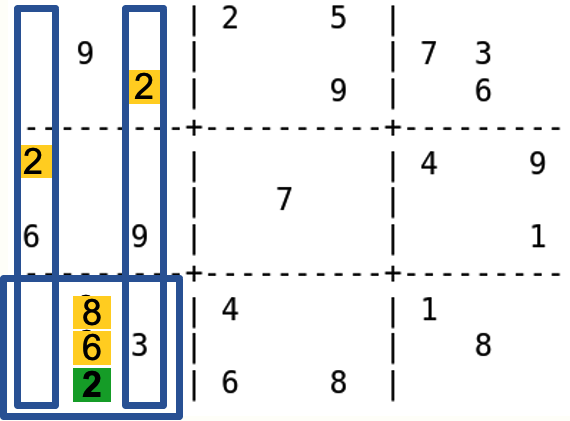
\includegraphics[width=0.8\textwidth]{figures/sudoku-step5}
\end{figure}
}
	\end{frame}

	\begin{frame}{Stepwise explanations for CSPs}
		\framesubtitle{EXPLANATION STEP}
%		In, we introduce \emph{explanation} steps \pause
		
      	Let an \emph{EXPLANATION STEP} (\citet{bogaerts2020step})  be:
      	
      	\begin{center}
      		{\Large {
\includegraphics[width=15pt]{figures/explanation_E}} $\&$ {
\includegraphics[width=15pt]{figures/explanation_S}} $\implies$ {
\includegraphics[width=15pt]{figures/explanation_N}}}
      	\end{center}
      	\pause
      \begin{minipage}{0.65\textwidth}
      	\begin{itemize}
      		\item[{
\includegraphics[width=15pt]{figures/explanation_E}}] A subset of previously derived facts ${E}$ 
      		\begin{itemize}
				\item[\textit{(Sudoku)}] Given and derived digits in the grid \pause
      		\end{itemize}
      		\item[{
\includegraphics[width=15pt]{figures/explanation_S}}] A minimal subset of model constraints 
      		\begin{itemize}
				\item[\textit{(Sudoku)}] Alldifferent column, row, box constraints \pause
			\end{itemize}

      		\item[{
\includegraphics[width=15pt]{figures/explanation_N}}] A newly derived fact s.t. ${E}' \& {S}' \implies n$
      	\end{itemize}
      \end{minipage}
        \begin{minipage}{0.34\textwidth}
			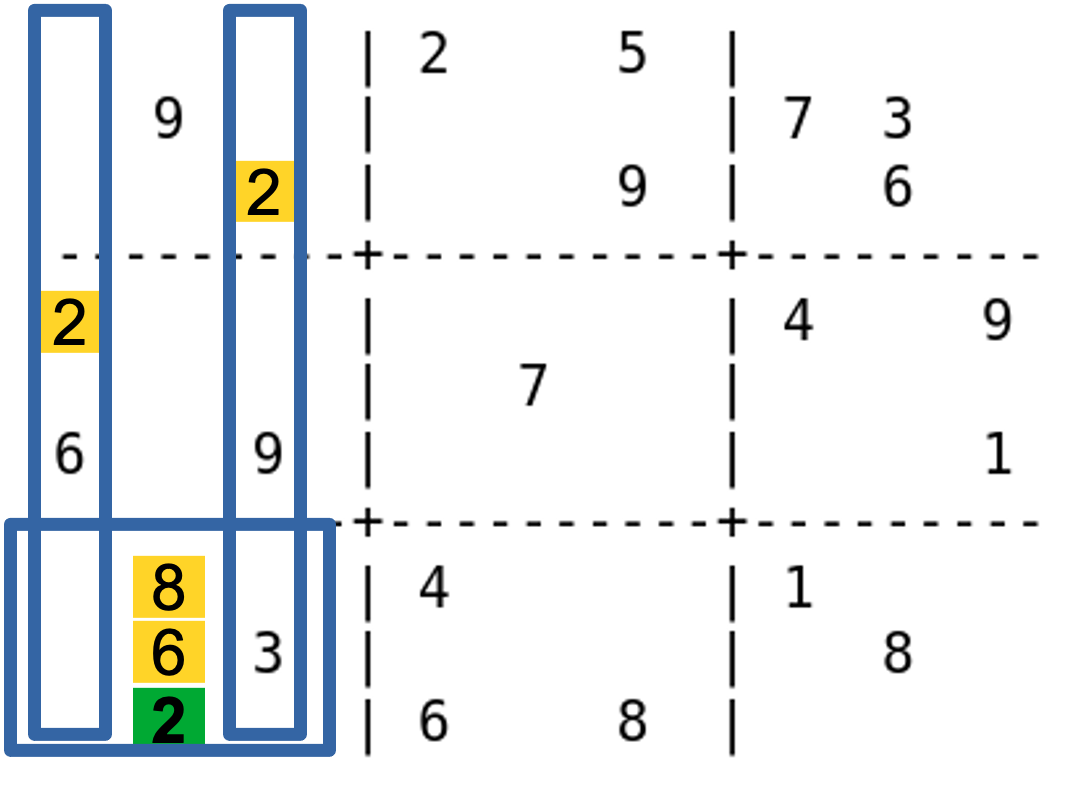
\includegraphics[width=\textwidth]{figures/sudoku3}
  \end{minipage}

\pause 
\begin{center}
{\Large \textbf{How ?} \pause \large $\mathtt{\mathbf{MUS}}($ 
\includegraphics[width=10pt]{figures/explanation_E_full} $\&$ {
\includegraphics[width=10pt]{figures/explanation_S_full}} $\& \lnot$ {
\includegraphics[width=10pt]{figures/explanation_N}} $)$ \textbf{is a valid explanation step}}
\end{center}

	\end{frame}
	
	
	\begin{frame}
		\frametitle{Stepwise explanations for CSPs}
		\framesubtitle{The best/easiest explanation step...}
%		\begin{center} 
			\textbf{What is a \emph{good} explanation ?} \pause \\
			Let $\mathbf{f}  ($ 
\includegraphics[width=10pt]{figures/explanation_E}, {
\includegraphics[width=10pt]{figures/explanation_S}}, {
\includegraphics[width=10pt]{figures/explanation_N}} $)$ be a cost-function that quantifies how good (e.g. easy to understand) an explanation step is.
			\pause 
		
		\vspace*{1cm}
		
		\hfill
	      \begin{minipage}{0.5\textwidth}
	      	\begin{center}
						\begin{algorithm}[H]

							$X_{best} \gets \mathit{nil}$\;
							\For{ n  $\in$ \texttt{propagate($S$)}}{
										
										$X \gets \call{MUS}{(S \land E \land \neg n)}$\;
										\uIf{$f(X)<f(X_{best})$}{
												$X_{best} \gets X$\;
											}
									}
								\Return{$X_{best}$} 
							\end{algorithm}
			
	      	\end{center}
		\end{minipage}
		\begin{minipage}{0.4\textwidth}
		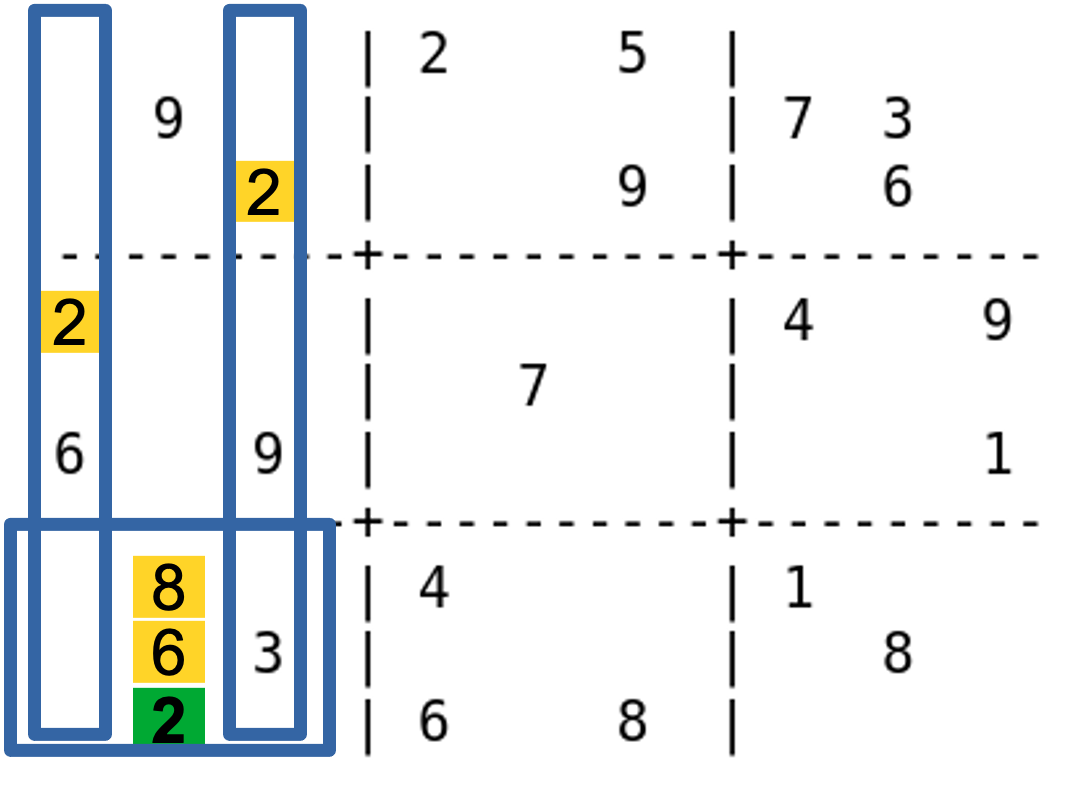
\includegraphics[width=\textwidth]{figures/sudoku3}
	\end{minipage}
%		\end{center}
	\end{frame}
	
	
	
	
	\section{Motivation}
	\begin{frame}{Motivation}
		\framesubtitle{Challenges and open questions from \cite{bogaerts2020step}}

		\begin{minipage}{0.53\textwidth}
%\begin{description}%[font=\color{vuborange}\itshape]
%	\item[Optimality] Explanations not provably optimal, \emph{heuristically} found.
%\end{description}
\emph{\textbf{Optimality}} w.r.t $\mathbf{f}$
	\begin{itemize}
		\item[$\triangleright$] MUS guarantees non-redundancy but ... not optimality.
		%				\item MUS-based heuristic
		\item[$\triangleright$] Alternative: SMUS $\#$-minimal (\cite{ignatiev2015smallest})
	\end{itemize} 
%\begin{description}[font=\color{vuborange}\itshape]
%	
%	\item[Efficiency] Explanation generation takes a lot of time: \pause
%	\begin{itemize}
%		\item[Q2] Can we avoid looping over the literals when searching for the next best explanation ?\pause
%		%					\begin{itemize}
%			%						\item[$\triangleright$] \emph{Constrainedness}
%			%					\end{itemize}
%		\item[Q3] Can we reuse information from an explanation call to another?
%		%				\begin{itemize}
%			%					\item[$\triangleright$] \emph{Incrementality}
%			%				\end{itemize}
%	\end{itemize}
%\end{description}
		\end{minipage}\hfill
	\begin{minipage}{0.42\textwidth}
		\begin{center}
			\begin{algorithm}[H]
				
				{\small $X_{best} \gets \mathit{nil}$\;
				\For{\color{black}  n  $\in$ \texttt{propagate($S$)}}{
					
					$X \gets \call{MUS}{(S \land E \land \neg n)}$\;
					\uIf{$f(X)<f(X_{best})$}{
						\emph{$X_{best} \gets X$}\;
					}
				}
				\Return{$X_{best}$} }
			\end{algorithm}
			
		\end{center}
	\end{minipage}
	
		%		\end{center}

		
	\end{frame}

	\begin{frame}{Motivation}
	\framesubtitle{Challenges and open questions from \cite{bogaerts2020step}}
	
	\begin{minipage}{0.53\textwidth}
		%\begin{description}%[font=\color{vuborange}\itshape]
		%	\item[Optimality] Explanations not provably optimal, \emph{heuristically} found.
		%\end{description}
		\emph{\textbf{Optimality}} w.r.t $\mathbf{f}$
		\begin{itemize}
			\item[$\triangleright$] MUS guarantees non-redundancy but ... not optimality.
			%				\item MUS-based heuristic
			\item[$\triangleright$] Alternative: SMUS $\#$-minimal (\cite{ignatiev2015smallest})
		\end{itemize} 
			Explanation generation takes a lot of time: 
%		\begin{description}[font=\color{vuborange}\itshape]
		%	
		%	\item[Efficiency] Explanation generation takes a lot of time: \pause
			\begin{itemize}
					\item[Q2] Can we \emph{avoid looping over the literals} when searching for the next best explanation ?\pause
			%		%					\begin{itemize}
				%			%						\item[$\triangleright$] \emph{Constrainedness}
				%			%					\end{itemize}
					\item[Q3] Can we \emph{reuse information} from an explanation call to another?
			%		%				\begin{itemize}
				%			%					\item[$\triangleright$] \emph{Incrementality}
				%			%				\end{itemize}
				\end{itemize}
		%\end{description}
	\end{minipage}
\hfill
	\begin{minipage}{0.42\textwidth}

			\begin{algorithm}[H]
				
				{\small $X_{best} \gets \mathit{nil}$\;
					\For{n  $\in$ \texttt{propagate($S$)}}{
						
						$X \gets \call{MUS}{(S \land E \land \neg n)}$\;
						\uIf{\color{black} $f(X)<f(X_{best})$}{
							$X_{best} \gets X$\;
						}
					}
					\Return{$X_{best}$} }
			\end{algorithm}
		
	\end{minipage}
	
	%		\end{center}


\end{frame}
	
	
	
	
	\section{The OCUS Problem}
			\begin{frame}{OCUS-Based explanation generation}
			\framesubtitle{The OCUS problem}
			\begin{definition}
				\small
				Let $\formula$ be a formula, $f:2^{\formula} \to \nat$ a cost function and  $p$ a predicate $p: 2^{\formula}\to \{\ltrue,\lfalse\}$. We call %a set $U\subseteq \formulag$ a \emph{$p$-constrained $f$-OUS} of \formulag ($(p,f)$-OUS) \tias{what with the OCUS name here?} \bart{I propsoe to say. We call 
					$\subsetT \subseteq \formula$ an \emph{OCUS}$^*$ of \formula (with respect to $f$ and $p$) if \begin{itemize}                                      
						\item $\subsetT$ is unsatisfiable,
						\item $p(\subsetT)$ is true
						\item \emph{all other unsatisfiable $\subsetT'\subseteq \formula$ with $p(\subsetT')=\ltrue$ satisfy $f(\subsetT')\geq f(\subsetT)$}.
					\end{itemize}
				\end{definition}
				$^*$ = Optimal \emph{Constrained} Unsatisfiable Subset
			\end{frame}
			
			
			
			\newcommand\onestepo{\ensuremath{\call{explain-One-Step-ocus}}\xspace}
			\begin{frame}{OCUS-Based explanation generation}

					\hspace{0.3\textwidth}
					\begin{minipage}{0.5\textwidth}
					\begin{algorithm}[H]
					$X_{best} \gets \mathit{nil}$\;
						\For{n  $\in$ \texttt{propagate($S$)}}{
							
							$X \gets \call{MUS}{(S \land E \land \neg n)}$\;
							\uIf{\color{black} $f(X)<f(X_{best})$}{
								$X_{best} \gets X$\;
							}
						}
						\Return{$X_{best}$} 
				\end{algorithm}
					\end{minipage} \pause

			\[\downarrow\]

				\hspace{0.17\textwidth}
					\begin{minipage}{0.8\textwidth}				
				\begin{algorithm}[H]
					\DontPrintSemicolon
					\emph{$p \leftarrow$ exactly one of $\{\lnot n \ | \ n \in \LitsToExplain\}$}\;
					$\call{OCUS}(S \wedge E \wedge \{\lnot n \ | \ n \in \LitsToExplain\}, \emph{f, p})$\;
				\end{algorithm}
								\end{minipage}

				
			\end{frame}

		\begin{frame}
		\begin{center}
			\Large
			\textbf{Q}: How to compute OCUSs?		
			
			
		\end{center}
			
			\end{frame}			
		
					
			\section{An OCUS algorithm: A hitting set-based algorithm}
			\subsection{Minimum hitting sets}
		
					\begin{frame}{Minimal Hitting set problem}
					\begin{itemize}
						\item Set of elements $\{c_1,c_2,...,c_n\}$ \pause
						\item Collection $\m{H}$ of sets-to-hit \pause
						\item \textbf{Goal}: Find the smallest hitting set such that every set-to-hit is hit at least once by an element of the hitting set. \pause
					\end{itemize}
					\vfill
					
					\begin{minipage}{0.48\textwidth}
						\only<4>{
							For example: 
							\begin{enumerate}
								\item[$H_1$] = $\{c_2, c_4, c_7\}$
								\item[$H_2$] = $\{c_3, c_5\}$
								\item[$H_3$] = $\{c_2, c_6\}$
								\item[$H_4$] = $\{c_1, c_8\}$
							\end{enumerate}
						}
						\only<5>{
							%			\color{gray}
							For example: 
							\begin{enumerate}
								\item[\color{gray}$H_1$]\color{gray} = $\{c_2, c_4, c_7\}$
								\item[\color{gray}$H_2$]\color{gray} = $\{c_3, c_5\}$
								\item[\color{gray}$H_3$]\color{gray} = $\{c_2, c_6\}$
								\item[\emph{$H_4$}]\emph{ = $\{c_1, c_8\}$}
							\end{enumerate}
						}
						\only<6>{
							
							For example: 
							\begin{enumerate}
								\item[\emph{$H_1$}] \emph{= $\{c_2, c_4, c_7\}$}
								\item[\color{gray}$H_2$]\color{gray} = $\{c_3, c_5\}$
								\item[\emph{$H_3$}] \emph{= $\{c_2, c_6\}$}
								\item[\color{gray}$H_4$]\color{gray} = $\{c_1, c_8\}$
							\end{enumerate}
						}
						\only<7>{
							For example: 
							\begin{enumerate}
								\item[\color{gray}$H_1$]\color{gray} = $\{c_2, c_4, c_7\}$
								\item[\emph{$H_2$}]\emph{ = $\{c_3, c_5\}$}
								\item[\color{gray}$H_3$]\color{gray} = $\{c_2, c_6\}$
								\item[\color{gray}$H_4$]\color{gray} = $\{c_1, c_8\}$
							\end{enumerate}
						}
					\end{minipage}
					\begin{minipage}{0.48\textwidth}
						%					\only<5>{
							%						Example hitting sets:
							%						\begin{itemize}
								%							\item $\{c_1, c_2, c_3\}$
								%							\item $\{c_8, c_2, c_5\}$
								%							\item \dots
								%						\end{itemize}
							%					}
						\only<5>{
							Example hitting sets:
							\begin{itemize}
								\item $\{$ \emph{$c_1$}$,  ...\}$ %c_2, c_3\}$
								
								%							\item $\{c_8, c_2, c_5\}$
								%							\item \dots
							\end{itemize}
						}
						\only<6>{
							Example hitting sets:
							\begin{itemize}
								\item $\{c_1, \emph{c_2}, ... \}$%, c_3\}$
								%							\item $\{c_8, c_2, c_5\}$
								%							\item \dots
							\end{itemize}
						}
						\only<7>{
							Example hitting sets:
							\begin{itemize}
								\item $\{c_1, c_2,$ \emph{$c_3$}$\}$
								%							\item $\{c_8, c_2, c_5\}$
								\item \dots
							\end{itemize}
						}
						
					\end{minipage}
					
					
				\end{frame}
			
			\subsection{Optimal Hitting Sets}
				
				\begin{frame}{\emph{Cost-Optimal} Hitting set problem}
					\begin{itemize}
						\item Set of elements $\{c_1,c_2,...,c_n\}$
						\item Collection $\m{H}$ of sets-to-hit\pause
						\item cost associated for every element:
						\[ w_1 =  \emph{3}, w_2= \emph{5}, w_3 = w_4 = ...= w_8 = 1\]\pause
						\item \textbf{Goal}: Find the \emph{optimal} hitting set such that every set-to-hit is hit by at least once an element of the hitting set with \emph{minimal total cost}.
					\end{itemize} \pause
					\vfill
					\begin{minipage}{0.48\textwidth}
						For example: 
						\begin{enumerate}
							\item[$H_1$] = $\{c_2, c_4, c_7\}$
							\item[$H_2$] = $\{c_3, c_5\}$
							\item[$H_3$] = $\{c_2, c_6\}$
							\item[$H_4$] = $\{c_1, c_8\}$
						\end{enumerate}
					\end{minipage}
					\begin{minipage}{0.48\textwidth}
						Optimal hitting sets:
						\begin{itemize}
							\item \st{$\{c_1, c_2, c_3\}$}
							\begin{itemize}
								\item cost: \emph{7}
							\end{itemize}
							\item $\{c_3, c_4, c_6, c_8\}$ \emph{\checkmark}
							\begin{itemize}
								\item cost: \emph{4}
							\end{itemize}
							\item \dots
						\end{itemize}
					\end{minipage}
				\end{frame}
			
			
			\subsection{Implicit Hitting Set Duality}
			\begin{frame}{An OCUS algorithm: A hitting set-based algorithm}
			\framesubtitle{Minimum Correction Subset vs Satisfiable Subsets}

			\only<1->{ Consider unsatisfiable  $\formula$ over atoms $x_1, x_2$:}
\only<2>{\[ c_1 := \lnot x_1 \vee \lnot x_2  \qquad  c_2 := \lnot x_1 \vee  x_2 \qquad c_3 := \lnot x_2  \qquad  c_4 := x_1\]}

\only<3>{\[ \emph{c_1 := \lnot x_1 \vee \lnot x_2  \qquad  c_2 := \lnot x_1 \vee  x_2 }  {\color{blue}\qquad c_3 := \lnot x_2  \qquad  c_4 := x_1}\]}

\only<4>{\[ c_1 := \lnot x_1 \vee \lnot x_2  \qquad  c_2 := \lnot x_1 \vee  x_2  \qquad c_3 := \lnot x_2  \qquad  \emph{   c_4 := x_1} \]}
		\only<3->{	\begin{definition}
				A set $C \subseteq \formula $ is a \only<3>{\emph{correction subset}}\only<4->{correction subset} of $\formula$ if \only<3>{{\color{blue} $ \formula \setminus \subsetT$}}\only<4->{ $ \formula \setminus \subsetT$} is satisfiable, a.k.a. Satisfiable Subset. \\
				\only<4->{A correction set $\subsetT$ is a \emph{minimum correction subset} if no strict subset $\subsetT' \subset \subsetT$ is also a correction set.}
			\end{definition} }
		\end{frame}
%
		\begin{frame}{An OCUS algorithm: A hitting set-based algorithm}
			\framesubtitle{Implicit Hitting set duality}
			
			\begin{itemize}
				\item[$\triangleright$] Exploit implicit hitting set--based duality between {\color{blue}MCSes} and {\color{teal}MUSes} (\cite{DBLP:journals/jar/LiffitonS08,ai/Reiter87})
			\end{itemize}\pause
			
			\begin{theorem}\label{prop:MCS-MUS-hittingset}
				%     
				A set  $\subsetT \subseteq \formula$ is a MCS of $ \formula$ iff  it is a \emph{minimal hitting set} of \muses{\formula}. \pause \\
				A set  $\subsetT \subseteq \formula$ is a MUS of $ \formula$ iff  it is a \emph{minimal hitting set} of \mcses{\formula}.
			\end{theorem} \pause
			\begin{itemize}
				\item[$\triangleright$] We extended this to OCUS: \pause
			\end{itemize}
			\begin{theorem}\label{prop:MCS-MUS-hittingset}
	%     
	A set  $\subsetT \subseteq \formula$ is an OCUS($ \formula, f, p)$ iff  it is a \emph{optimal hitting set} of \mcses{\formula} that satisfies $p$.
\end{theorem}		
		
		\end{frame}
		
		
			
			
			%\begin{frame}{An OCUS algorithm: A hitting set-based algorithm}
			%	\framesubtitle{Implicit Hitting set duality}
			%	
			%	\begin{minipage}{0.65\textwidth}
				%		%     
				%		A set  $\subsetT \subseteq \formula$ is a MCS of $ \formula$ iff  it is a \emph{minimal hitting set} of \muses{\formula}.\\
				%		A set  $\subsetT \subseteq \formula$ is a MUS of $ \formula$ iff  it is a \emph{minimal hitting set} of \mcses{\formula}.
				%	\end{minipage}
			%\end{frame}
			
			
		
		
		
		
			\begin{frame}{An OCUS algorithm: A hitting set-based algorithm}
				


					\begin{algorithm}[H]
						\caption{$\comus(\formula,f,p)$ }
						\label{alg:comus}
						\DontPrintSemicolon
						$\setstohit  \gets \emptyset$ \tcp*{ Collection of sets-to-hit} \pause %\label{omus-line1} 
						\While{\color{black} true}{
							$\subsetT \gets \emph{\cohs(\setstohit,f,p)} $ \; \pause%\tcp*{\small Find \textb    $\setstohit  \gets \setstohit  \cup \{  \formula \setminus \F''\}$ \;
								% f{optimal} solution}
							% \tcp{\small set with all unique clauses from hitting set}
							%     (sat?, $\kappa$) $\gets$ \texttt{SatSolver}($hs$)\;
							% \tcp{If SAT, $\kappa$ contains the satisfying truth assignment}
							% \tcp{IF UNSAT, $hs$ is the OUS }
							\If{\color{black} $\lnot \sat(\subsetT)$}{
								\Return{\color{teal}$\subsetT$} \tcp*{ OCUS found!}
							}\pause
							$\setstohit  \gets \setstohit \ \cup $ {\color{blue}$\corrss(\subsetT,\formula)$} 
						}
					\end{algorithm}
	\pause \vfill
	{\color{blue}$\corrss(\subsetT,\formula)$} 
	\begin{itemize}
		\item $\{  \formula \setminus \subsetT\}$ \pause
		\item   $\{  \formula \setminus \grow(\subsetT, \formula)\}$  \pause $\rightarrow$ \textit{ {\color{blue} efficient vs qualitative grow ?}} \pause
		\item Multiple correction subsets ? 
	\end{itemize}
				%\end{minipage}
				
			\end{frame}
			
			%\begin{frame}{An OCUS algorithm: A hitting set-based algorithm}
			%	
			%	{\SetAlCapFnt{\small}
				%		\small
				%		\begin{algorithm}[H]
					%			\DontPrintSemicolon
					%			$\setstohit  \gets \emptyset$ \tcp*{\footnotesize Collection of sets-to-hit} %\label{omus-line1} 
					%			\While{\color{black} true}{
						%				$\subsetT \gets \emph{\cohs(\setstohit,f,p)} $ \tcp*{\footnotesize hitting set}%\tcp*{\small Find \textb    $\setstohit  \gets \setstohit  \cup \{  \formula \setminus \F''\}$ \;
							%				% f{optimal} solution}
						%				% \tcp{\small set with all unique clauses from hitting set}
						%				%     (sat?, $\kappa$) $\gets$ \texttt{SatSolver}($hs$)\;
						%				% \tcp{If SAT, $\kappa$ contains the satisfying truth assignment}
						%				% \tcp{IF UNSAT, $hs$ is the OUS }
						%				\If{\color{black} $\lnot \sat(\subsetT)$}{
							%					\Return{\color{teal}$\subsetT$} \tcp*{\footnotesize OCUS found!}
							%				}
						%				$\subsetT \gets  \grow(\subsetT,\formula) $ \label{line:grow}\tcp*{\footnotesize Grow Satisfiable subset}
						%				$\setstohit  \gets \setstohit \ \cup $ {\color{blue}$\{  \formula \setminus \subsetT\}$} \tcp*{\footnotesize Add correction subset (new set-to-hit)}
						%			}
					%			\caption{\small$\comus(\formula,f,p)$ }
					%			\label{alg:comus}
					%		\end{algorithm}
				%	}
			%	%\end{minipage}
			%	
			%\end{frame}
			
			\section{Open questions and challenges}
			
			\begin{frame}{Improving efficiency of our OCUS algorithm..}
				\framesubtitle{...in the context of explanation sequence generation}
				
				\begin{center}
					\large
					Can we \emph{improve} OCUS-calls in the \emph{context of explanation generation} ? 
				\end{center} \pause
				\begin{minipage}{0.5\textwidth}
				\begin{figure}[H]
					\centering
					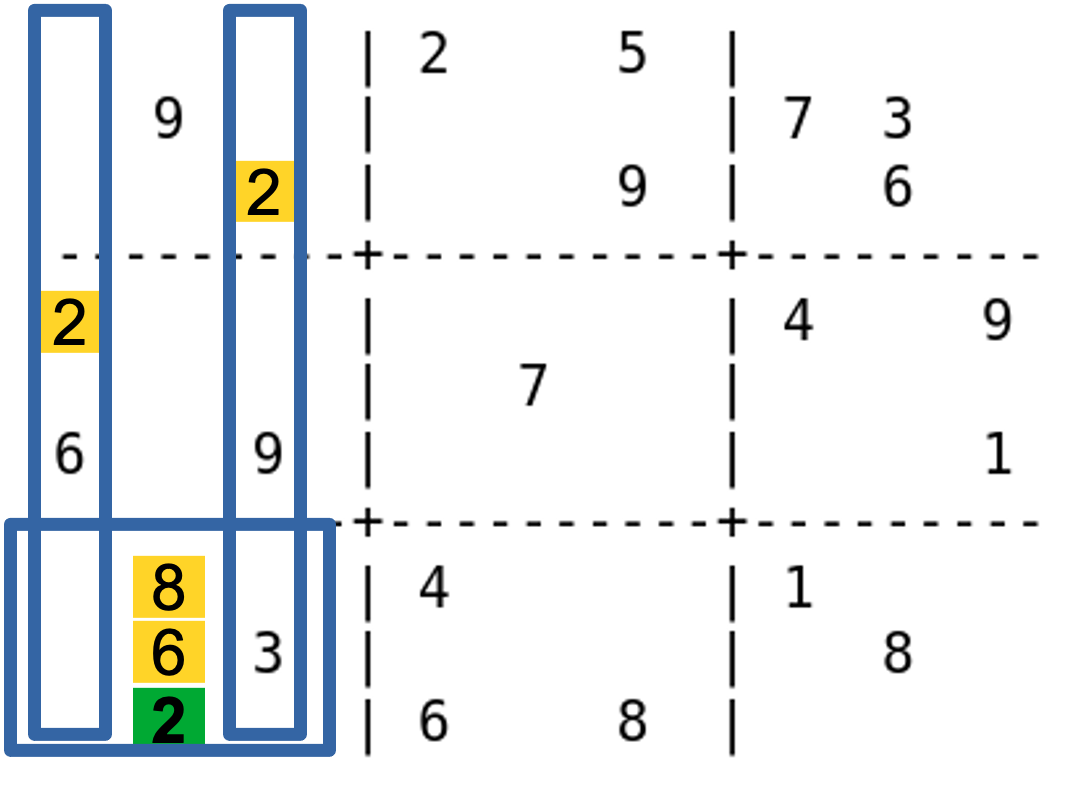
\includegraphics[width=0.8\textwidth]{figures/sudoku3}
				\end{figure}
			\end{minipage}
			\begin{minipage}{0.49\textwidth}
				\begin{center}
					{\Large $\mathtt{\mathbf{MUS}}($ 
\includegraphics[width=10pt]{figures/explanation_S_full} $\&$ {
\includegraphics[width=10pt]{figures/explanation_E_full}} $\& \lnot$ {
\includegraphics[width=10pt]{figures/explanation_N}} $)$ }
				\end{center}				
\begin{itemize}
	\item[{
\includegraphics[width=15pt]{figures/explanation_S_full}}] A minimal subset of model constraints \pause
	\begin{itemize}
		\item \emph{Does not change} from an explanation step to another \pause
	\end{itemize}
	\item[{
\includegraphics[width=15pt]{figures/explanation_E_full}}] A subset of previously derived facts ${E}$  \pause
	\begin{itemize}
		\item \emph{Precision-increasing !}
	\end{itemize}
	
\end{itemize}		
	
	\end{minipage}
		
		
				
			\end{frame}
			
			
			
			
			\begin{frame}{Incrementality}
				
					\begin{algorithm}[H]
						
						\DontPrintSemicolon
						\emph{\bf  $\setstohit  \gets \dots$} \tcp*{\emph{Collection of sets to hit}}
						\While{\color{gray} true}{
							$\subsetT \gets \cohs(\emph{\setstohit},f,p) $  \;
							\color{gray}
							\If{\color{gray} $\lnot \sat(\subsetT)$}{
								\Return{\color{gray}$\subsetT$} \tcp*{OCUS found!}
							}
							{\color{black}$\setstohit  \gets \setstohit  \cup \emph{ \corrss( \subsetT, \formula)}$ } \;
						}
						\caption{$\comus(\formula,f,p)$ }
						\label{alg:comus}
					\end{algorithm}
				\pause
				\vfill
				\begin{itemize}
					\item[$\triangleright$] Keep track of collection of correction sets $\m{H}$ that need to be hit \pause
					\item[$\triangleright$] Each set H in \m{H} is the complement (with respect to the formula at hand) of a \emph{satisfiable subset} \pause
					\begin{itemize}
						\item[$\rightarrow$] Keep track of \emph{set of Satisfiable Subsets \textbf{SSs}} \pause
						\item[$\rightarrow$] Bootstrap $\m{H} \gets \{\m{F} \setminus \m{S} | \m{S}  \in  \mathbf{SSs} \}$ 
					\end{itemize}
					
					
				\end{itemize}
				
			\end{frame}
			
		\begin{frame}
			\frametitle{Outline}
			\tableofcontents
		\end{frame}
		
		\section{Results}
		
		\begin{frame}{Results - Explanation quality}

				\begin{figure}
				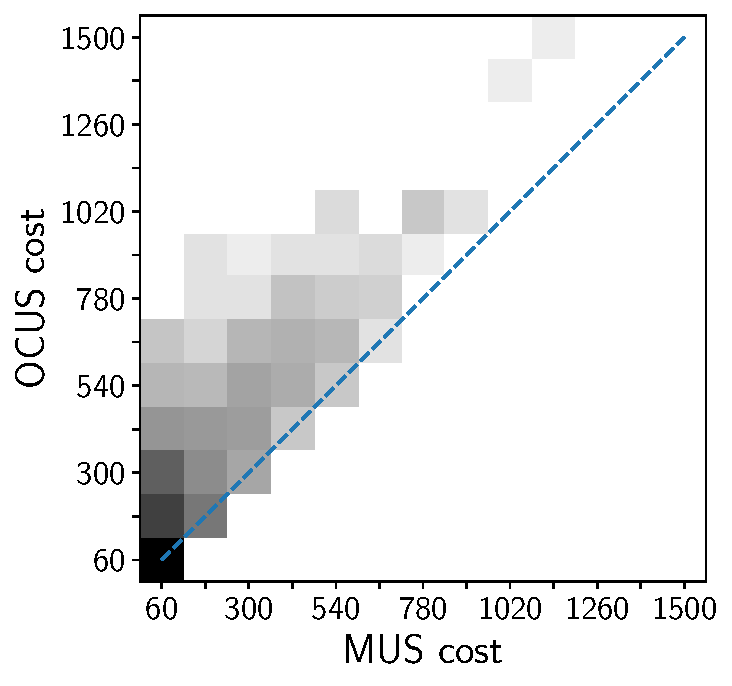
\includegraphics[width=0.6\textwidth]{figures/heatmapcosts_ocus_mus_2022040412.pdf}
					\end{figure}

		\end{frame}
		
		\begin{frame}{Results - Correction Subset Enumeration}
			\begin{minipage}{0.59\textwidth}
				\begin{figure}[H]
	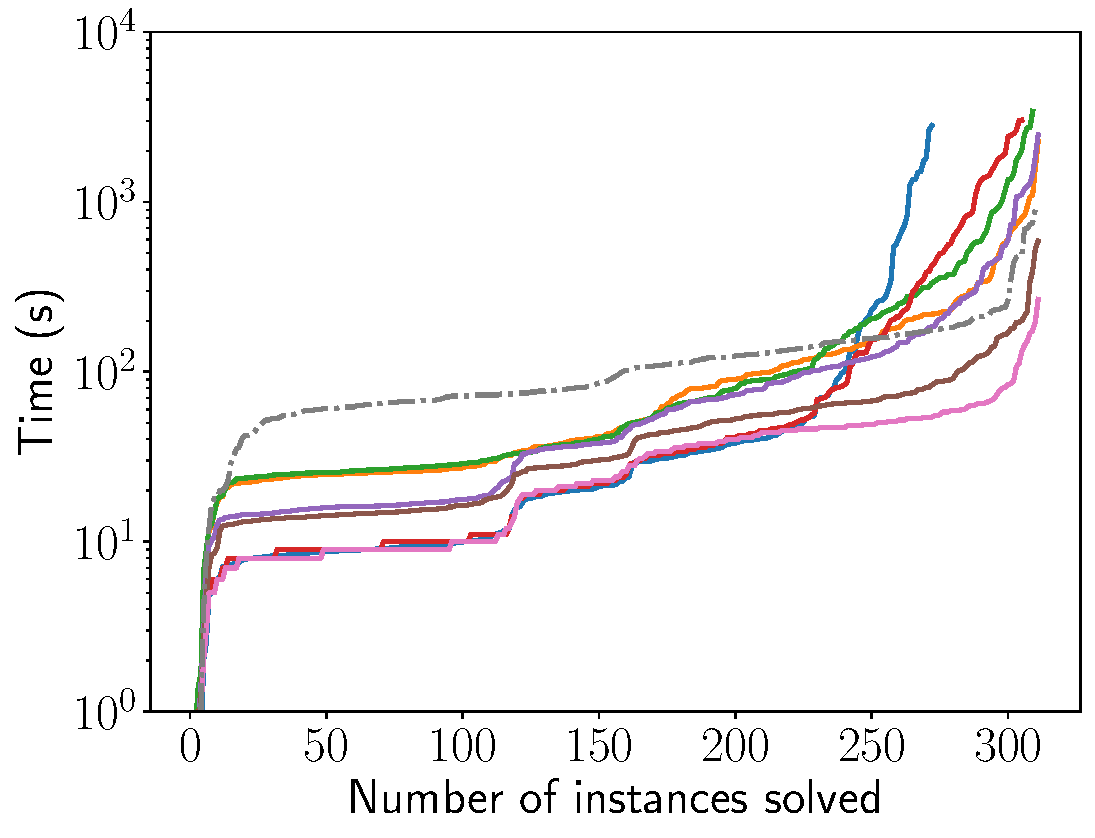
\includegraphics[width=\textwidth]{figures/rq2_cactus_log_2022_06_27_OUS_IterLit_Incr_HS.pdf}
\end{figure}

			\end{minipage}
			\begin{minipage}{0.4\textwidth}
				\begin{figure}[H]
	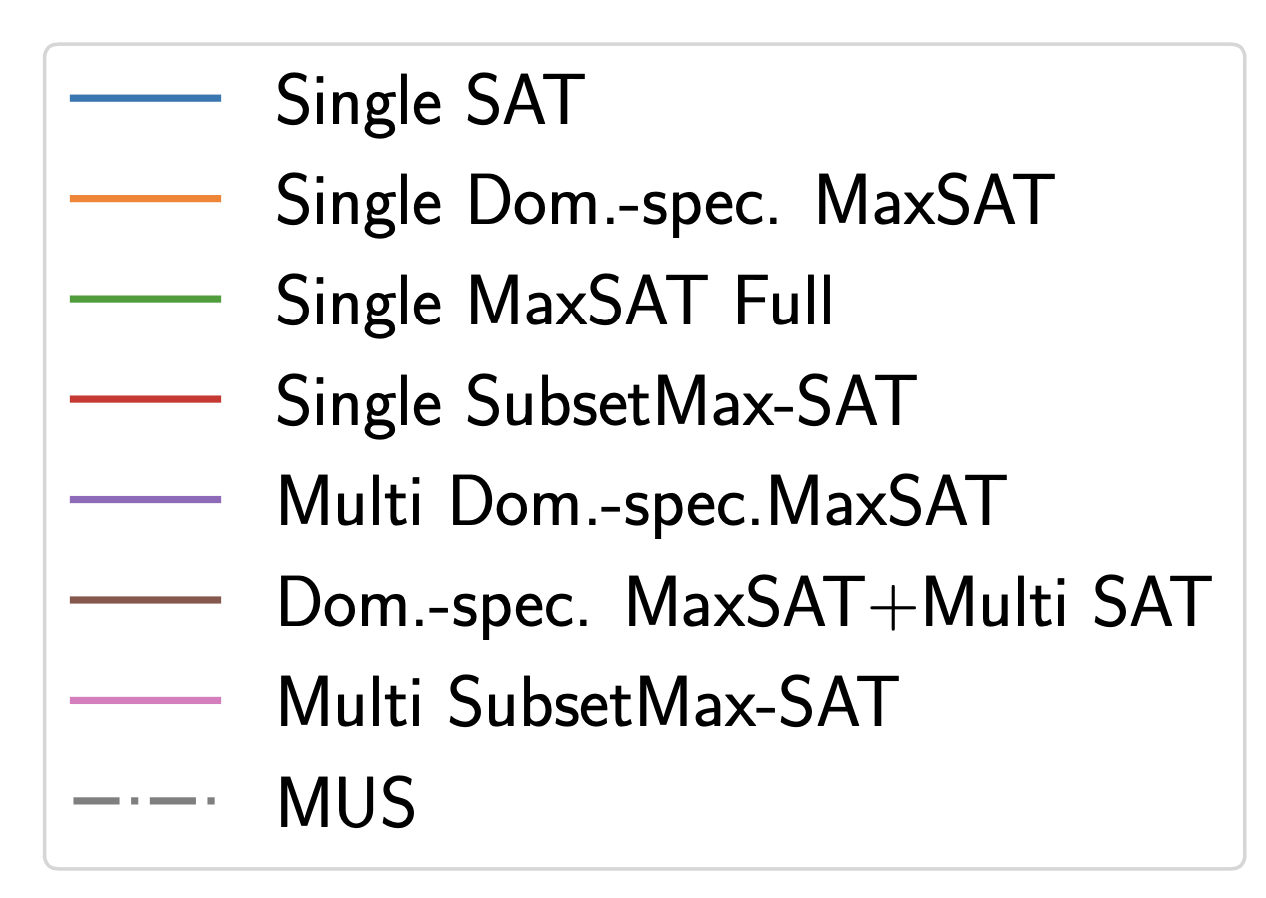
\includegraphics[width=0.9\textwidth]{figures/grow_types}
\end{figure}
\end{minipage}
		\end{frame}
		
		
		\begin{frame}{Results - Incrementality}
			%	\framesubtitle{Explanation configurations compared}
	\begin{figure}
	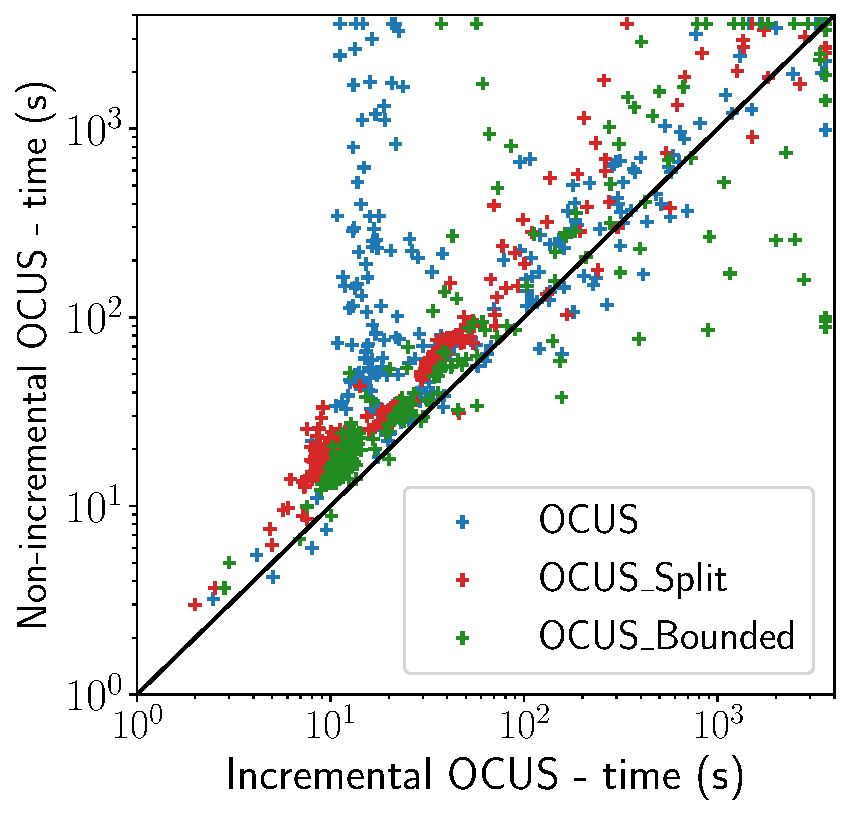
\includegraphics[width=0.6\textwidth]{figures/incremental_vs_non_SAT_2022_06_22.pdf}
\end{figure}
		\end{frame}
		
		
		\section{Conclusion and Future work}
		\begin{frame}{Conclusion}
			In this paper, we introduce (cost-)\emph{\underline{O}ptimal \underline{C}onstrained} \underline{U}nsatisfiable \underline{S}ubsets (OCUS) problem and solved it using the \emph{implicit hitting set duality} between {\color{blue}MCSes} and {\color{teal}MUSes}.
			\vfill
			\begin{description}
				\item[Optimality] Cost-function quantifies explanation difficulty. \pause
				\item[Constrainedness] Analyze structural constraints on the form of the explanations.\pause
				\item[Incrementality] Reuse-information between successive explanation calls.
				%		\item[Efficiency] 
				%		\begin{enumerate}
					%			\item Explanation-specific grow;
					%			\item Bound and sort OUS calls
					%		\end{enumerate}
			\end{description}
			\vfill
		\end{frame}
		
		
		\begin{frame}{Use cases}
				\begin{center}\Large
					What can OCUS do for YOU ? 
				\end{center}
				\begin{figure}
					\centering
					
\includegraphics[width=0.2\textwidth]{figures/i_want_you_ocus.png}
				\end{figure}\pause
				\begin{itemize}
					\item Cost-optimal Constrained Unsatisfiable Subsets \pause
					\item Stepwise explaining unsatisfiability \pause
				\item Explaining scheduling, configuration problems .... and puzzles  \Cooley
					\item Explaining Optimality for Constraint Optimization Problems 
					\begin{itemize}
						\item Why is the objective value not better ? 
					\end{itemize}


				\end{itemize}
			\end{frame}
		
		\begin{frame}{Future work}
			
			\begin{itemize}
				\item[$\triangleright$] Learning the optimization function (from humans)
				\item[$\triangleright$] Explaining optimization (different types of ``why'' queries); close relation to Explainable AI Planning \cite{fox2017explainable}
				\item[$\triangleright$] Scaling up (approximate algorithms; decomposition of explanation search)
%				\item[$\triangleright$] Incremental algorithms over different ``why'' queries
				% \item 
			\end{itemize}	
			
			
		\end{frame}
		
		
		\begin{frame}
			\begin{center}
				{\huge Questions?}
			\end{center}		
		\end{frame}
		
		
		\begin{frame}[allowframebreaks]
			\frametitle{References}
			\bibliographystyle{named}
			\bibliography{refs}
		\end{frame}
		
		
		
	\end{document}
	
	
	
	
	
	
	
	
	
